\section{Säure, Basen und pH-Wert}

\subsubsection{Definition}
\begin{tabular} {l l}
 Säuren geben Protonen (H+) ab & Basen nehmen Protonen auf \\
\end{tabular}

\subsubsection{Säure-Base GGW}
$\rightarrow$ Tabelle liest man von links nach rechts \newline
\begin{minipage}{0.65\columnwidth}
	Bergab = GGW rechts: \ce{ HCl + H2O <=>> Cl- + H3O+ }
	
	Bergauf = GGW links: \ce{ HS- + H2O <<=> S^{2-} + H3O+ }
\end{minipage}

\subsection{pH-Wert}
\begin{itemize}
	\item pH < 7, sauer (mehr $\ce{H3O^+}$ als $\ce{OH^-}$)
	\item pH = 7, neutral (reines Wasser bei 25$^{\circ}$C)
	\item pH > 7, basisch (mehr $\ce{OH^-}$ als $\ce{H3O^+}$)
\end{itemize}
\subsubsection{neutralisation}
Prinzip der Neutralisation = Saure und basische lösungen können sich gegenseitig neutralisieren. \newline
Konzentration von $\ce{OH^- und H3O^+}$ berechnen und \textbf{pH Wert berechnen (pH = 14 - pOH)} \newline
$\ce{
	\textcolor{red}{H3O+ (aq)} + Cl^- (aq) + Na+ (aq) + \textcolor{blue}{OH^- (aq)}
	-> \textcolor{violet}{2 H2O (l)} + Na+ (aq) + Cl^- (aq)
}$
% Salpetersäure + Natronlauge → Wasser + Kochsalzlösung


\subsection{Protolyse - Säure, Base Reaktion}
\begin{enumerate}
	\item Welche ist Säure, welche Base? (welches nimmt H, welches gibt H)
	\item Reagiert es? -> Säure und Base reagieren dann miteinander, wenn sie in Bergab-Stellung stehen (GGW rechts), ansonsten ist sie nicht stark.
	\item Reaktionsgleichung aufstellen
	\item H zur konjugierten Säure hinzufügen und von Säure entziehen.
	\item Ladungen überprüfen (negative Ladung = mehr Elektronen als Protonen und positive Ladung = weniger Elektronen als Protonen)
\end{enumerate}

\begin{center}
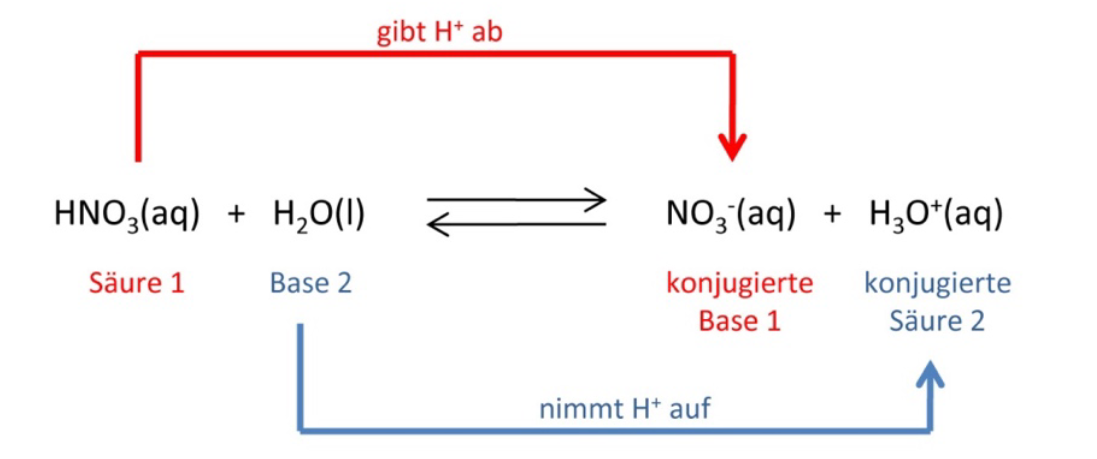
\includegraphics[scale=0.2]{images/Saure_Base_ex.png}
\end{center}
